\begin{figure*}[t]
    \centering
    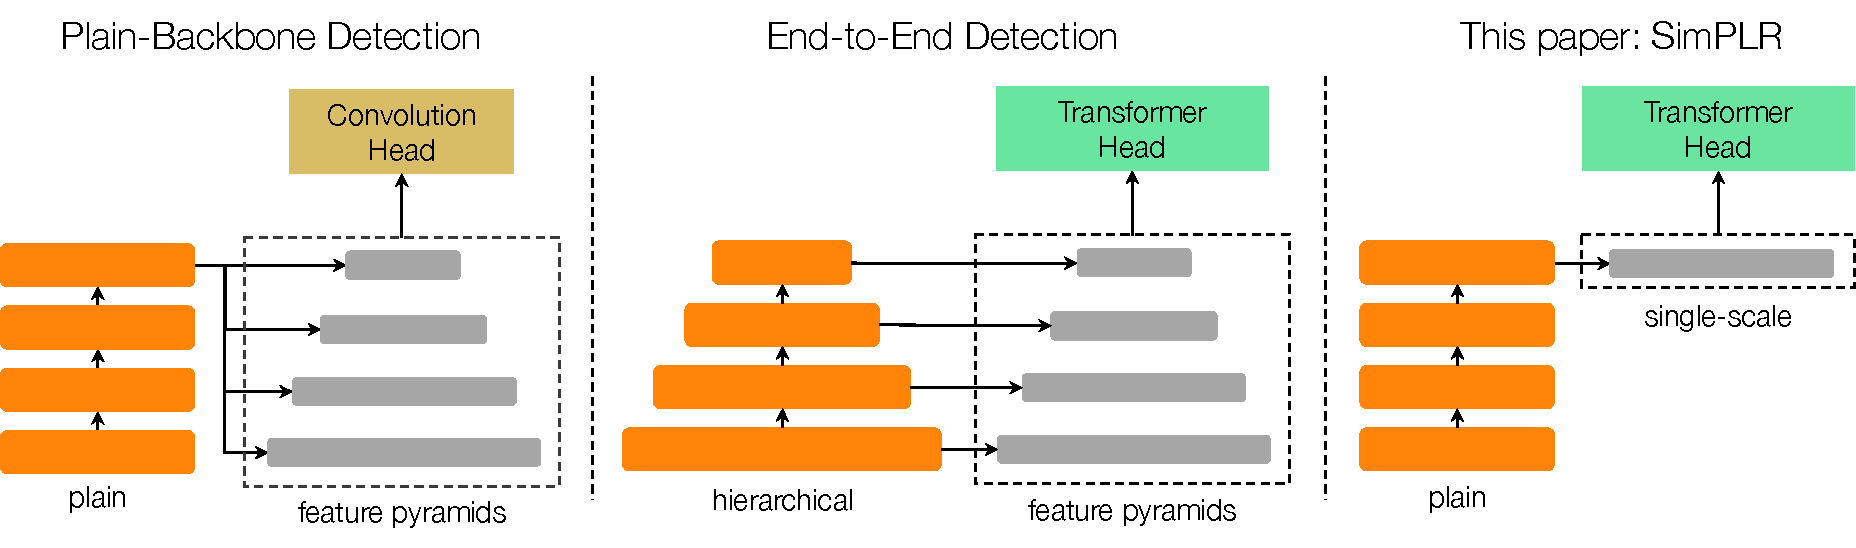
\includegraphics[width=\linewidth]{fig/compare1.pdf}\\
    \caption{
    \textbf{Object detection architectures. Left:} The plain-backbone detector from~\cite{li2022vitdet} whose input (denoted in the dashed region) are multi-scale features. \textbf{Middle:} State-of-the-art end-to-end detectors~\cite{nguyen2022boxer,cheng2022mask2former} utilize a hierarchical backbone (\ie, Swin~\cite{liu2021swintransformer}) to create multi-scale inputs. \textbf{Right:} Our simple single-scale detector following the end-to-end framework. Where existing detectors require feature pyramids to be effective, we propose a plain detector, \ours, whose backbone and detection head are non-hierarchical and operate on a single-scale feature map. The plain detector, \ours, achieves on par or even better performance compared to hierarchical and/or multi-scale counterparts while being more efficient.
    % We show through our experiments that \ours also shows good scaling behaviour and effectively takes advantages from a significant progress of self-supervised learning with ViTs.
    }\label{fig:compare}
\end{figure*}

\section{\ours: A Simple and Plain Detector}
\label{sec:simplr}

Multi-scale feature maps in a hierarchical backbone can be easily extracted from the pyramid structure~\cite{wei2016ssd,tsung2017fpn,zhu2021deformable}. When moving to a ViT backbone with a constant feature resolution, the creation of multi-scale feature maps requires complex backbone adaptations. Moreover, the benefits of multi-scale features in object detection frameworks using ViTs remain unclear. Recent studies on plain-backbone detection~\cite{li2022vitdet,chen2022uvit} conjecture the high-dimensional ViT with self-attention and positional embeddings~\cite{vaswani2017transformer} is able to preserve important information for localizing objects\footnote{ViT-B and larger ($\text{dim}\ge768$) can maintain information with a patch size of $16{\times}16{\times}3$ in the input image.}. From this conjecture, we hypothesize that a proper design of the transformer-based head will enable a plain detector.

Our proposed detector, \ours, is conceptually simple: a pre-trained ViT backbone to extract plain features from an image, which are then fed into a single-scale encoder-decoder to make the final prediction (See \cref{fig:compare}). Thus, \ours is a natural idea as it eliminates the non-trivial creation of feature pyramids from the ViT backbone. But the single-scale encoder-decoder requires an effective design to deal with objects at different scales. Next, we introduce the key elements of \ours, including its \emph{scale-aware} attention that is the main factor for learning of adaptive object scales.

\subsection{Scale-aware attention}

The output features of the encoder should capture objects at different scales. Therefore, unlike the feature pyramids where each set of features encode a specific scale, predicting objects from a plain feature map requires its feature vectors to reason about dynamic scale information based on the image content. This can be addressed effectively by a multi-head attention mechanism that capture different scale information in each of its attention heads. 
In that case, global self-attention is a potential candidate because of its large receptive field and powerful representation. However, its computational complexity is quadratic \wrt the sequence length of the input, making the operation computationally expensive when dealing with high-resolution images. The self-attention also leads to worse performance and slow convergence in end-to-end detection~\cite{zhu2021deformable}. This motivated us to develop a multi-head \emph{scale-aware} attention mechanism based on sparse attention such as box-attention and deformable attention.

\boldparagraph{Scale-aware box-attention (SAB).} The multi-head attention mechanism, proposed by~\cite{vaswani2017transformer}, is a core operation in the transformer architectures for capturing diverse patterns given a query vector in the input features. In the multi-head box-attention~\cite{nguyen2022boxer}, each feature vector is assigned a reference window which is then refined to locate a region-of-interest in each attention head via scaling and translation transformations. Theoretically, the scaling transformation should provide box-attention the capability to learn multi-scale regions-of-interest in multiple attention heads. However, we find in our experiments that the scaling function in box-attention only performs minor modifications regarding to its reference window. As a result, feature vectors learn to adapt to a specific scale of the reference window assigned to them. While this behaviour may not impact the multi-scale box-attention -- which utilizes feature pyramids for detecting objects -- it poses a big challenge in learning scale-equivariant features on a single-scale input.

To address this limitation, we propose two variants of multi-head \emph{scale-aware} attention (\ie, \emph{fixed-scale} and \emph{adaptive-scale}) that integrate different scales into each attention head, allowing query vectors to choose the suitable scale information during training. Our proposed attention mechanism is simple: we assign reference windows of $m$ different scales to attention heads of each query. We use $m$ reference windows with size $w {=} h \in \{s \cdot 2^j\}_{j=0}^{m-1}$, where $s$ is the size of the smallest window, and $m$ is the number of scales. Surprisingly, our experiments show that the results are not sensitive to the size of the window, as long as \emph{enough number of scales} are used.
%
\begin{enumerate}[leftmargin=*,itemsep=0pt,topsep=0pt]
    \item[i)] \emph{Fixed-Scale Attention.} Given reference windows of $m$ scales, we distribute them to $n$ attention heads in a round-robin manner. Thus, in multi-head fixed-scale attention, $\frac{n}{m}$ attention heads are allocated for each of the window scales. This uniform distribution of different scales enables fixed-scale attention to learn diverse information from local to more global context. The aggregation of $n$ heads results in scale-aware features, that is suitable for predicting objects of different sizes.
    \item[ii)] \emph{Adaptive-Scale Attention.} Instead of uniformly assigning $m$ scales to $n$ attention heads, the adaptive-scale attention learns to allocate a scale distribution based on the context of the query vector. This comes from the motivation that the query vector belonging to a small object should use more attention heads for capturing fine-grained details rather than global context, and vice versa. 
    
    % More specifically, in each attention head, the adaptive-scale attention predicts offsets for all reference windows of $m$ scales and samples feature grids from $m$ regions-of-interest. 
    % Given the query vector $q \in \mathbb{R}^d$, it then applies a learnable projection on $q$ followed by $\softmax$ normalization to generate attention scores which allow it to focus on the feature grid of suitable scale. The adaptive-scale attention provides efficiency due to sparse sampling and strong flexibility to control scale distribution via its attention computation.
    Given the query vector $q \in \mathbb{R}^d$ in the input feature map and $m$ reference windows of different scales, $\{r^j\}_{j=0}^{m-1}$, the adaptive-scale attention predicts offsets of all reference windows, $\{\Delta_{x_j},\Delta_{y_j},\Delta_{w_j},\Delta_{h_j}\}_{j=0}^{m-1}$, in each attention head. Besides, we apply a scale temperature to each set of offsets before the transformations:
    \begin{equation}
        F_\text{scale}(r_j, q) = [x, y, w + \Delta_w\cdot\frac{2^j}{\lambda}, h + \Delta_h\cdot\frac{2^j}{\lambda}], 
    \end{equation}
    \begin{equation}
        F_\text{translate}(r_j, q) = [x + \Delta_x\cdot\frac{2^j}{\lambda}, y + \Delta_y\cdot\frac{2^j}{\lambda}, w, h],
    \end{equation}
    where $\frac{2^j}{\lambda}$ is the scale temperature corresponding to $r_j$. The scale temperature allows the transformation functions to capture regions of interest corresponding to the scale of reference windows. It then samples feature grids from $m$ regions of interest and generates attention scores for these feature grids followed by $\softmax$ normalization. This makes our attention mechanism to focus on feature grids of suitable scale. The adaptive-scale attention provides efficiency due to sparse sampling and strong flexibility to control scale distribution via its attention computation.
\end{enumerate}

\boldparagraph{Scale-aware deformable attention (SAD).} Here, we adopt deformable attention to capture information of $m$ scales. Instead of $4$ sampled points per query, we predict $4\cdot m$ points around the query coordinate. Each set of $4$ points is first initialized at the corners of square whose center is the query coordinate and size is increased by a factor of 2. Similar to adaptive-scale box-attention, we apply a scale temperature to each set of offsets before the deformable function, yielding adaptive-scale deformable attention. This encourages each set of points to attend to regions corresponding to its scale.

\subsection{Network Architecture} 

\ours follows the end-to-end detection and segmentation framework in~\cite{nguyen2022boxer} with the two-stage design. Specifically, we use a plain ViT as the backbone with $14\times14$ windowed attention and four equally-distributed global attention blocks as in~\cite{li2022vitdet}. In the detection head, the \ours encoder receives input features via a projection of the last feature map from the ViT backbone. The object proposals are then generated using single-scale features from the encoder and top-scored features are initialized as object queries for the \ours decoder to predict bounding boxes and masks. 

% Note this design differs from most state-of-the-art systems~\cite{cheng2022mask2former,li2022vitdet,lin2023plaindetr}, where the feature pyramids are essential for object proposal generation and/or final prediction. Our approach follows the spirit of ViT~\cite{dosovitskiy2021vit} that applies a single and constant feature resolution throughout the detection head, which turns out to largely simplify the architectural choices and remove handcrafted components compared to Swin~\cite{liu2021swintransformer} or MViT~\cite{fan2021mvit}.

Formally, we apply a projection $f$ to the last feature map of the pre-trained ViT backbone, resulting in the input feature map $e \in \mathbb{R}^{H_e \times W_e \times d}$ where $H_e, W_e$ are the size of the feature map, and $d$ is the hidden dimension of the detection head. In \ours, the projection $f$ is simply a single convolution projection, that provides us a great flexibility to control the resolution and dimension of the input features $e$ to the encoder. The projection allows \ours to decouple the feature scale and dimension between its backbone and detection head to further improve the efficiency. This practice is different from the creation of SimpleFPN in~\cite{li2022vitdet} where a different stack of multiple convolution layers is used for each feature scale (more details shown in Fig. A in the supplementary material). We show by experiments that this formulation is key for plain detection and segmentation while keeping our network efficient.

\boldparagraph{Plain backbone.} \ours deploys ViT as its plain backbone for feature extraction. We show that \ours can take advantages of recent progress in self-supervised learning with ViTs. To be specific, \ours generalizes to ViT backbones initialized by MAE~\cite{he2022mae} and BEiTv2~\cite{peng2022beitv2}. The efficient design of \ours allows us to effectively scale to larger ViT backbones which recently show to be even more powerful in learning representations~\cite{he2022mae,zhai2022scalingvit,dehghani2023scalingvit22b}. We also provide the comparison between different pre-training approaches in the supplementary material.

\boldparagraph{Adaption for panoptic segmentation.} Panoptic segmentation proposed by~\cite{kirillov2019panoptic} requires the network to segment both ``thing'' and ``stuff''.
To enable the plain detector on panoptic segmentation, we make an adaptation in the mask prediction of \ours. Following~\cite{cheng2022mask2former}, we predict segmentation masks of both types by computing the dot-product between object queries and a feature map. We provide a brief description on these modifications, the full implementation details are provided in the supplementary material.

In~\cite{cheng2022mask2former}, the $\frac{1}{4}$ feature scale is extracted from the first stage of the Swin and combined with upscaled $\frac{1}{8}$ features from the last layer of the encoder for the mask prediction. As the ViT and SimPLR encoder features are of lower resolution, we simply interpolate the last encoder layer to $\frac{1}{4}$ scale and add a single attention layer on top. This simple modification produces a high resolution feature map that is beneficial for learning fine-grained details.
%
Masked instance-attention follows the dense grid sampling strategy (\ie, $14\times14$ feature grid) of box-attention in the decoder~\cite{nguyen2022boxer}, but differs in the computation of the attention scores to better capture objects of different shapes. Inspired by masked self-attention~\cite{cheng2022mask2former}, we employ the masking to $14\times14$ attention scores of the feature grid based on the mask prediction scores in the previous decoder layer. By focusing better on foreground features, the decoder yields more discriminative features.

% Our goal is to have \emph{minimal} adaptation which allows us to use the same training recipe for all tasks, including object detection, instance segmentation, and panoptic segmentation. As the output feature of our encoder is in $\frac{1}{8}$ scale of the original image, we simply use a transposed convolution layer to generate the high-resolution feature for mask prediction. We found that it is beneficial to stack $K$ encoder layers on top of the high-resolution feature to learn more contextual information. In addition, we incorporate the decoder with masked instance-attention to obtain discriminative representation for mask prediction. Different from masked cross-attention in~\cite{cheng2022mask2former}, our masked instance-attention extends box-attention in~\cite{nguyen2022boxer} which yields a small complexity when dealing with feature map of $\frac{1}{8}$ scale from the encoder. More details are provided in the supplementary document.

% \boldparagraph{Masked instance-attention.} The masked instance-attention follows the grid sampling strategy of the box-attention in~\cite{nguyen2022boxer}, but differs in the computation of attention scores to better capture objects of different shapes. To be specific, the region of interest $r'_i$ is divided into 4 bins of $2 \times 2$ grid, each of which contains a $\frac{m}{2} \times \frac{m}{2}$ grid features sampled using bilinear interpolation. Instead of assigning an attention weight to each feature vector, a linear projection ($\mathbb{R}^d \rightarrow \mathbb{R}^{2 \times 2}$) is adopted to generate the $2 \times 2$ attention scores for 4 bins. The $\frac{m}{2} \times \frac{m}{2}$ feature vectors within the same bin share the same attention weight. This is equivalent to the \textit{average} aggregation of feature values covered by each bin, which shows to reduce misalignments in RoIAlign~\cite{he2017maskrcnn}:
% \begin{equation}
%     \mathrm{head}_i = \sum_{k=0}^{2 \times 2} \sum_{j=0}^{\frac{m}{2} \times \frac{m}{2}} \frac{\alpha_k}{\frac{m}{2} \cdot \frac{m}{2}} \, v_{i_{k,j}},
% \end{equation}
% where $a_k$ is the attention weight corresponding to $k$-th bin and $v_{i_{k,j}}$ is the $j$-th feature vector inside $k$-th bin.


% Inspired by~\cite{cheng2022mask2former}, we utilize the mask prediction before the $\sigmoid$ of the previous decoder layer $\mathcal{M}_q \in \mathbb{R}^{H_m \times W_m}$ corresponding to the object query $q$. Given the coordinates of grid features within the region of interest $r'_i$, we sample the corresponding mask scores using bilinear interpolation. The sampled mask scores are binarized with the 0.5 threshold and applied into the attention computation.
% %
% \begin{align}
%     \mathrm{head}_i &= \sum_{k=0}^{2 \times 2} \sum_{j=0}^{\frac{m}{2} \times \frac{m}{2}} \Big(\frac{\alpha_k}{\frac{m}{2} \cdot \frac{m}{2}} + m_{i_{k,j}} \Big) \, v_{i_{k,j}} , \\
%     m_{i_{k,j}} &= 
%         \begin{cases}
%         0 & \text{if } \sigmoid\Big(\mathcal{M}_q\big(v_{i_{k,j}}\big)\Big) \geq 0.5 \\
%         -\infty & \text{otherwise} \\
%         \end{cases}   ,
% \end{align}
% %
% where $\mathcal{M}_q\big(v_{i_{k,j}}\big)$ is the mask score sampled at the location of the feature $v_{i_{k,j}}$. The masked instance-attention along with high-resolution layers allow \ours to capture more fine-grained details, which is beneficial for panoptic segmentation.
